% !TeX program = lualatex

\documentclass{article}
\usepackage[a4paper, total={6in, 10in}]{geometry}
\usepackage[utf8]{inputenc}
\usepackage{mathtools}
\usepackage[english]{babel}
\usepackage{amsthm}
\usepackage{amsfonts}
\usepackage{calrsfs}
\usepackage{lmodern}%get scalable font
\usepackage{titling}
\usepackage{listings}
\usepackage{fancyhdr}
\usepackage{graphicx}
\usepackage[dvipsnames]{xcolor}
\usepackage{fontspec}
\usepackage{lstfiracode}
\usepackage{tikz}
\usetikzlibrary{trees}

% Define command for show :=
\newcommand{\defeq}{\vcentcolon=}
% Set font family
\fontfamily{qpl}\selectfont 
% Calligraphic H
\DeclareMathAlphabet{\pazocal}{OMS}{zplm}{m}{n}
\newcommand{\Hb}{\pazocal{H}}
\newcommand{\Bb}{\pazocal{B}}

\newcommand*{\QEDB}{\null\nobreak\hfill\ensuremath{\square}}


\newtheorem{theorem}{Theorem}
\newtheorem{corollary}{Corollary}[theorem]
\newtheorem{lemma}[theorem]{Lemma}
\newtheorem{fact}[theorem]{Fact}
\newtheorem{definition*}[theorem]{Definition}

\title{Eight hands-on: Count-min sketch: range queries\\[1ex] \large Algorithm Design (2021/2022)}
\author{Gabriele Pappalardo\\Email: g.pappalardo4@studenti.unipi.it\\Department of Computer Science}
\date{April 2022}

\pretitle{
    \begin{center}
    \LARGE
    \includegraphics[width=5cm]{/Users/gabryon/Projects/Papers/AD-21-22/assets/images/unipi.png}\\
}
\posttitle{
    \end{center}
}

\setmonofont{FiraCode}[
    Scale=0.85,
    Contextuals=Alternate % Activate the calt feature
]

\lstset{
    style=FiraCodeStyle,
    breakatwhitespace=false,         
    breaklines=true,                 
    captionpos=b,                    
    keepspaces=true,                
    showspaces=false,                
    showstringspaces=false,
    basewidth=0.6em,
    showtabs=false,                  
    tabsize=2,
    frame=single,
    basicstyle=\ttfamily, % Use \ttfamily for source code listings
    commentstyle=\color{ForestGreen}
}


\setcounter{section}{0}

\begin{document}

\maketitle

\section{Introduction}

Consider the counters $F[i]$ for $1 \le i \le n$, where $n$ is the number of items in the stream of any length. 
At any time, we know that $|| F ||$ is the total number of items (with repetitions) seen so far, where each 
$F[i]$ contains how many times the item $i$ has been so far.  
We saw that CM-sketches provide a FPTAS $F'[i]$ such that $F[i] \le F'[i] \le F[i] + \varepsilon  ||F||$, 
where the latter inequality holds with probability at least $1 - \delta$.\newline

\noindent Consider now a range query $(a,b)$, where we want $F_{ab} = \sum_{a \le i \le b} F[i]$. Show how to adapt CM-sketch so that a FPTAS $F'_{ab}$ is provided: 

\begin{itemize}
    \item Baseline is $\sum_{a \le i \le b} F'[i]$, but this has drawbacks as both time and error grows with $b-a+1$.
    \item Consider how to maintain counters for just the sums when $b-a+1$ is any power of $2$ (less or equal to $n$):
    \begin{itemize}
        \item Can we now answer quickly also when $b-a+1$ is not a power of two? 
        \item Can we reduce the number of these power-of-2 intervals from $n \log n$ to $2n$?
        \item Can we bound the error with a certain probability? \textit{Suggestion}: it does not suffice to say that it is at most $\delta$ 
        the probability of error of each individual counter; while each counter is still the actual wanted value plus the residual as before, 
        it is better to consider the sum $V$ of these wanted values and the sum $X$ of these residuals, and apply Markov’s inequality to $V$ and $X$ 
        rather than on the individual counters.  
    \end{itemize} 
\end{itemize}

\section{Solution}

\subsection{Baseline Solution}

The baseline solution is pretty straightforward to implement: we can use a \verb+for+ loop starting from the element $a$ up to $b$ and sum
all the counters. Since each counter has some error, if we sum up all the counter in a large range,
then also the final error will grow linearly as large as the range, that is $b - a + 1$.

\begin{lstlisting}[language=Python,caption=`Range query for integer values']
def range(F: CountMinSketch, a: int, b: int): int:
    sum = 0
    for i in range(a, b + 1):
        sum += F[i]
    return sum
\end{lstlisting}

\subsection{Requested Solution}

\noindent We can improve the baseline solution using ranges of powers of two. In fact, any range $(a, b)$ can be
expressed as disjoint union of length with the powers of two, e.g., if we have the range $(4, 10)$:
$$
(4, 10) = (4) \cup (5, 8) \cup (9, 10)
$$

\noindent We can state the following fact that will allow us to compute all the possible range queries.

\begin{fact}[Dyadic Ranges]
    Any range in the interval from $1$ to $n$ is expressible as the disjoint union of $2 \log n$ intervals 
    in the set of dyadic ranges.
\end{fact}

\noindent Therefore, given a universe $U$ we can build a collection of \textit{dyadic ranges}, and we will
need at most $2n$ of them. Having these ranges, we can bind the error of the range query up to $\log n$, thus a
logarithmic error.

\begin{equation*}
    F_{ab} \le \tilde{F}_{ab} \le F_{ab} + 2 \varepsilon \log{n} ||F||
\end{equation*}

\noindent This can be achieved using $\log n$ Count-Min Sketches. We build a ``logic'' binary tree where each range is split in two parts.
Starting from the root we represent the range $(1, n)$ and going down we will have $(1, n/2)$ and $(n/2 + 1)$. We repeat the splitting process
until we are not able to do so anymore, that is, when we obtain $n$ ranges of the form $(1,1), (2, 2), (3, 3), \dots, (n-1, n-1), (n, n)$.
In each level of this ``logic'' binary tree we add a new Count-Min Sketch, having in total $\log n$ sketches.

\begin{figure}[htp]
    \centering
    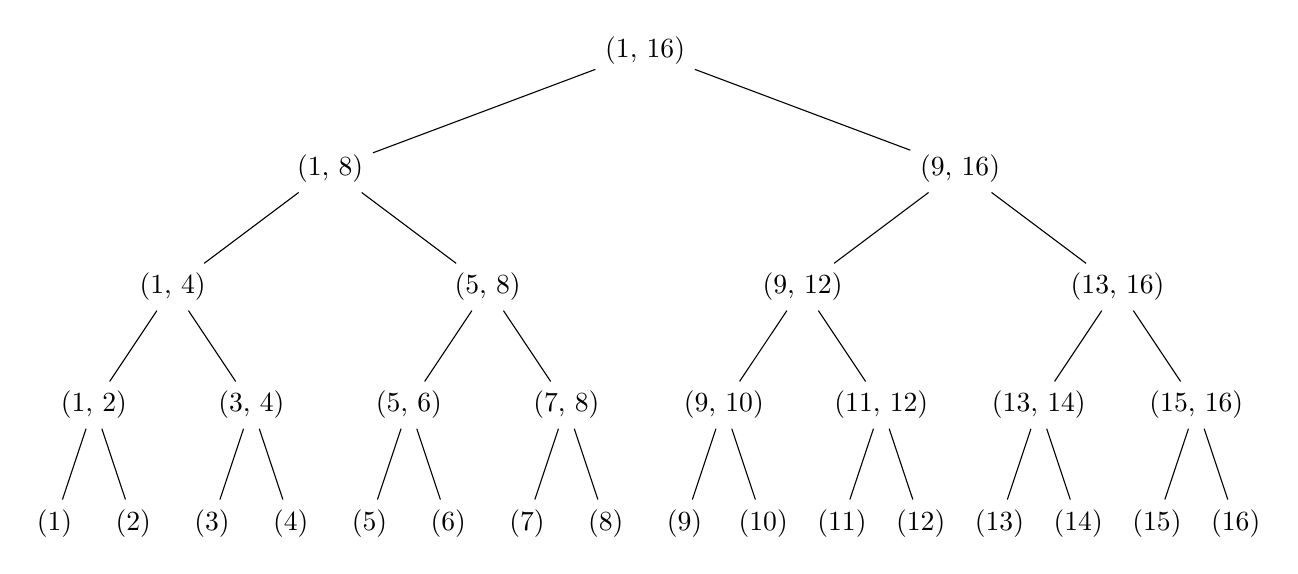
\begin{tikzpicture}[
        level distance=1.5cm, 
        level 1/.style={sibling distance=8cm}, 
        level 2/.style={sibling distance=4cm}, 
        level 3/.style={sibling distance=2cm},
        level 4/.style={sibling distance=1cm}
    ]
        \node {(1, 16)}
            child {
                node {(1, 8)}
                child {
                    node {(1, 4)}
                    child {
                        node {(1, 2)}
                        child {node {(1)}}
                        child {node {(2)}}
                    }
                    child {
                        node {(3, 4)}
                        child {node {(3)}}
                        child {node {(4)}}
                    }
                }
                child {
                    node {(5, 8)}
                    child {
                        node {(5, 6)}
                        child {node {(5)}}
                        child {node {(6)}}
                    }
                    child {
                        node {(7, 8)}
                        child {node {(7)}}
                        child {node {(8)}}
                    }
                }
            }
            child {
                node {(9, 16)}
                child {
                    node {(9, 12)}
                    child {
                        node {(9, 10)}
                        child {node {(9)}}
                        child {node {(10)}}
                    }
                    child {
                        node {(11, 12)}
                        child {node {(11)}}
                        child {node {(12)}}
                    }
                }
                child {
                    node {(13, 16)}
                    child {
                        node {(13, 14)}
                        child {node {(13)}}
                        child {node {(14)}}
                    }
                    child {
                        node {(15, 16)}
                        child {node {(15)}}
                        child {node {(16)}}
                    }
                }
            };
    \end{tikzpicture}
    \caption{Generated ranges using $n = 16$.}
\end{figure}
   
\noindent When we have to update a counter, we traverse the tree updating the counters for each traversed range.
For instance, if we have to update the counter for the element $7$ in Figure 1, we are going to update the counters
in each range containing the element, that are: $(1, 16), (1, 8), (5, 8), (7, 8), (7)$. 
The \verb+update+ operation takes $O(\log n)$ time, the pseudo-Python code is shown in Listing below.

\begin{lstlisting}[language=python]
def update(x: int) -> None:
    # The first range to update is the root
    range = (1, n)
    level = 1
    # When the range has size one we stop
    while range != (x, x):
        # Update the CMS in the current level
        update(CMSS[level], range) 
        # Go a level below in the logical tree
        level += 1 
        # Compute the new range to update
        if x in (range[0], int(range[1]/2)):
            range = (range[0], int(range[1] / 2))
        else:
            range = (int(range[0] / 2) + 1, range[1])
    return
\end{lstlisting}

\noindent The \verb+query+ operation relies on \textbf{Fact} 1, also this computation takes $O(\log n)$ time. 
We have to select each dyadic range needed to build the original range.

\begin{lstlisting}[language=python]
def query(r: (int, int)) -> int:
    sum = 0
    # Assuming we have a function that computes
    # dyadic ranges.
    ranges = dyadicRanges(r)
    # Query each CMS in the respective level with
    # the computed ranges
    for (level, range) in ranges:
        sum += normal_query(CMSS[level], range)
    return 0
\end{lstlisting}

\noindent These algorithms work also with one Count-Min Sketch, the universe of the counters will be the dyadic ranges.

\subsection{Bounding the failure probability}

The error analysis will require some definitions to work with. First, we are going to define the set of dyadic ranges as:
\begin{equation*}
    D = \{(1, n), (1, {n}/{2}), ({n}/{2} + 1, n), \dots, (1, 1), (2, 2), \dots, (n, n)\}, |D| = 2n
\end{equation*}

\noindent The analysis makes use of $\log n$ Count-Min Sketches as stated before, and it is restricted to the ranges contained in the set $D$. Furthermore, we
introduce the function:
\begin{equation*}
    \textrm{dy}: \mathcal{P}(\mathbb{N} \times \mathbb{N}) \to \mathcal{P}(D) 
\end{equation*}
which computes the dyadic ranges of a given range, as described in the previous section. For any range $r$ given to the function $\textrm{dy}$, thanks to the \textbf{Fact} 1, we have that:
\begin{equation*}
    \forall r \in \mathcal{P}(\mathbb{N} \times \mathbb{N}). |\textrm{dy}(r)| \le 2 \log n
\end{equation*}

\noindent We express the counter $F_{i}$ where the range $i = (a, b) \in D$. The approximate counter $\tilde{F}_{i}$ is obtained
as follows in Equation 1.

\begin{equation}
    \tilde{F}_{i} = F_{i} + X_i
\end{equation}

\noindent The random variable $X_{i}$ is a value representing the ``garbage'' (according to the definition given during the lectures). We would like to know the expected value of this random variable.
To do so, we define a new indicator random variable, as seen in class:
\begin{equation*}
    I_{j,i,k} = \begin{cases}
        1 & h_j(i) = h_j(k) \\
        0 & \textrm{othwerwise}
    \end{cases} \; i, k \in D, j \in [d]
\end{equation*}

\noindent Therefore, when the $j$-th hash function has a collision with different ranges in $D$ the variable will be set to $1$. 
Fixed a $j \in [d]$ and given an $i \in D$ we can define $X_{i}^{(j)}$ as: 

\begin{equation*}
    X_{i}^{(j)} = \sum_{k \in \textrm{dy}(i)}I_{j, i, k} \cdot  F_k
\end{equation*}

\noindent We can compute its expectation as follows:

\begin{equation*}
    \begin{split}
        E\bigg[X_{i}^{(j)}\bigg] & = E\bigg[\sum_{k \in \textrm{dy}(i)}I_{j, i, k} F_k\bigg] \\
        & = \sum_{k \in \textrm{dy}(i)} E[I_{j, i, k} \cdot F_k] \\
        & = \sum_{k \in \textrm{dy}(i)} \textrm{Pr}(\{I_{j, i, k} = 1\}) F_k \\
        & = \sum_{k \in \textrm{dy}(i)} \frac{\varepsilon}{e} \cdot  F_k \\ 
        & = \frac{\varepsilon}{e} \sum_{k \in \textrm{dy}(i)} F_k \\
        & \le \frac{\varepsilon}{e} 2 \log n ||F||
    \end{split}
\end{equation*}

\noindent Knowing that $E\big[X_{i}^{(j)}\big] \le 2 \log n \frac{\varepsilon}{e} ||F||$, we can bind the error probability in a single row using the Markov's inequality:

\begin{gather*}
    \textrm{Pr}(\{\tilde{F}_{i} \ge F_{i} + \varepsilon 2 \log n ||F||\}) \le \delta \iff \\
    \textrm{Pr}\bigg(\bigg\{F_{i} + X_{i} \ge F_{i} + \varepsilon 2 \log n ||F|| \bigg\}\bigg) \le \delta \iff \\
    \textrm{Pr}\bigg(\bigg\{X_i \ge 2 \varepsilon \log n ||F||\bigg\}\bigg) \le \frac{E\big[ X_i \big]}{\varepsilon 2 \log n ||F||} = \frac{2\log n \frac{\varepsilon}{e} ||F||}{\varepsilon 2 \log n ||F||} = \frac{1}{e}
\end{gather*}

\noindent Since we have $d$ row, where each hash function is independent, we will have:

\begin{equation*}
    \prod_{j \in [d]} \textrm{Pr}\bigg(\bigg\{ X_{i}^{(j)} \ge 2 \varepsilon \log n ||F||\bigg\}\bigg) \le \bigg(\frac{1}{e}\bigg)^d = \delta
\end{equation*}

\end{document}
